\documentclass{article}

\usepackage{graphicx}
\usepackage{tikz}
\usepackage{tikzsymbols}
\usetikzlibrary{calc,patterns,shapes.geometric}
\pagestyle{empty}
\usepackage[margin=0pt]{geometry}
\geometry{papersize={14in,12in}}

\def\centerarc[#1](#2)(#3:#4:#5){\draw[#1] ($(#2)+({#5*cos(#3)},{#5*sin(#3)})$) arc (#3:#4:#5);}

\begin{document}
	\begin{figure}
		\centering
		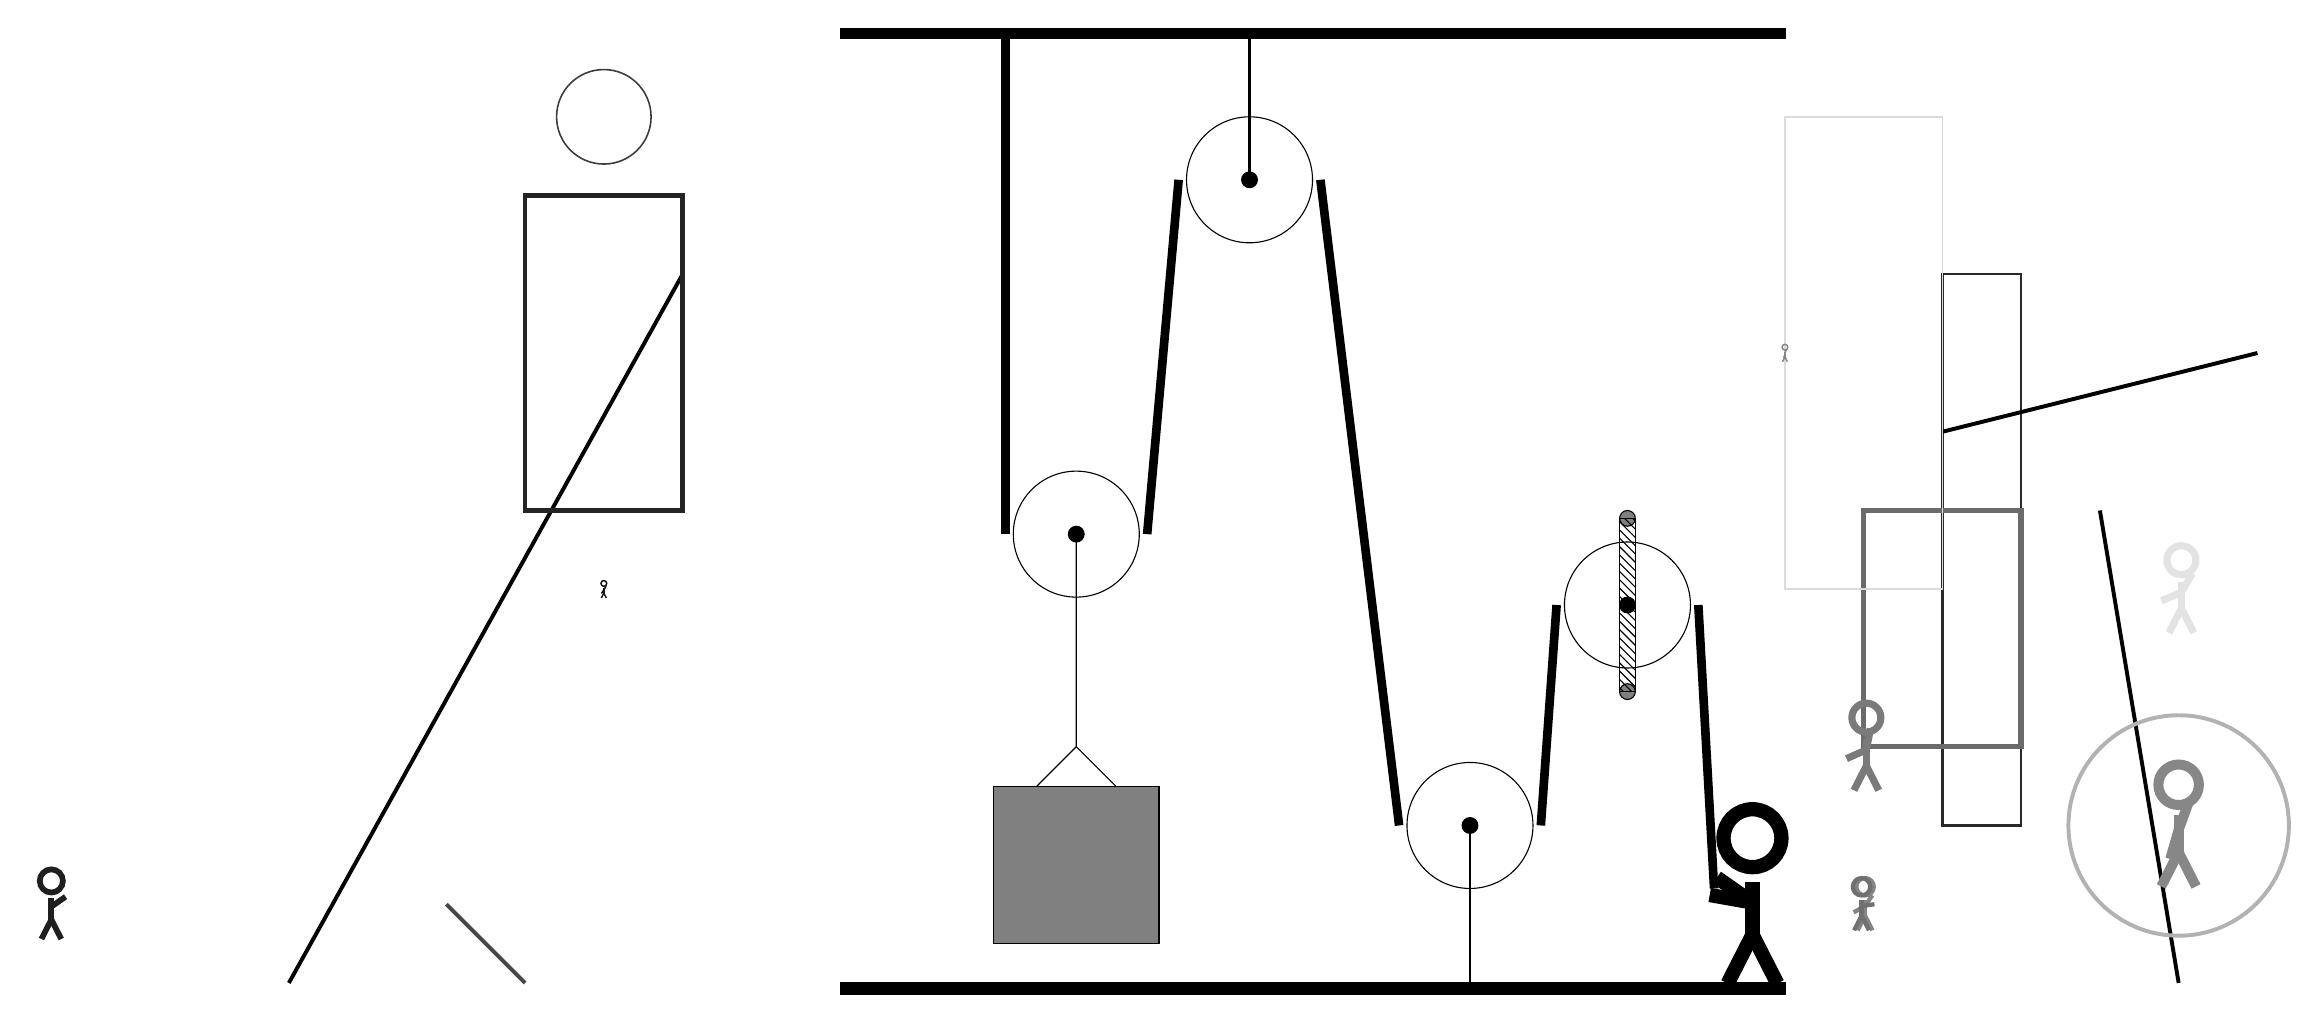
\begin{tikzpicture}
			%%%%% START %%%%%
			
			\draw[fill=black] (-2, 9) rectangle (10, 9.125);
			
			\draw (1, 2.7) circle (0.8);
			\draw[fill=black] (1, 2.7) circle (0.1);
			
			\draw (3.2, 7.2) circle (0.8);
			\draw[fill=black] (3.2, 7.2) circle (0.1);
			\draw[thick] (3.2, 7.2) -- (3.2, 9);
			
			\draw (6, -1) circle (0.8);
			\draw[fill=black] (6, -1) circle (0.1);
			\draw[thick] (6, -1) -- (6, -3);
			
			\draw[fill=white](8, 1.8) circle (0.8);
			\draw[fill=black] (8, 1.8) circle (0.1);
			\draw[fill=black!50] (8, 2.9) circle (0.1);
			\draw[fill=black!50] (8, 0.7) circle (0.1);
			\draw[pattern=north west lines, pattern color=black] (7.9, 2.9) rectangle (8.1, 0.7);
			
			\draw (1, 2.7) -- (1, 0) -- (0.5, -0.5);
			\draw (1, 0) -- (1.5, -0.5);
			\draw[fill=black!50] (-0.05, -0.5) rectangle (2.05, -2.5);
			
			\draw[line width=1.1mm] (0.1, 9) -- (0.1, 2.7);
			\centerarc[line width=1.1mm](1, 2.7)(180:360:0.9);
			\draw[line width=1.1mm](1.9, 2.7) -- (2.3, 7.2);
			\centerarc[line width=1.1mm](3.2, 7.2)(0:180:0.9);
			\draw[line width=1.1mm](4.1, 7.2) -- (5.1, -1);
			\centerarc[line width=1.1mm](6, -1)(180:360:0.9);
			\draw[line width=1.1mm](6.9, -1) -- (7.1, 1.8);
			\centerarc[line width=1.1mm](8, 1.8)(0:180:0.9);
			\draw[line width=1.1mm](8.9, 1.8) -- (9.1, -1.8);
			
			\draw[line width=0.5mm, color=black!99](14, 3) -- (15, -3);
			
			\node[line width=0.4mm, color=black!48] at (11, -2) {\Strichmaxerl[3][29][56]};
			\draw [line width=0.5mm, color=black!30](15, -1) circle (1.4);
			\draw[line width=0.3mm, color=black!84] (12, 6) rectangle (13, -1);
			\draw[line width=0.7mm, color=black!58] (11, 3) rectangle (13, 0);
			\draw[line width=0.5mm, color=black!99](-4, 6) -- (-9, -3);
			\draw [line width=0.2mm, color=black!77](-5, 8) circle (0.6);
			
			\draw[line width=0.5mm, color=black!100](12, 4) -- (16, 5);
			\node[line width=0.4mm, color=black!56] at (11, -2) {\Strichmaxerl[3][89][8]};
			\draw[line width=0.5mm, color=black!72](-6, -3) -- (-7, -2);
			
			\node[line width=0.7mm, color=black!47] at (15, -1) {\Strichmaxerl[7][74][70]};
			\node[line width=0.7mm, color=black!11] at (15, 2) {\Strichmaxerl[5][23][60]};
			\node[line width=0.7mm, color=black!52] at (11, 0) {\Strichmaxerl[5][24][79]};
			
			\node[line width=0.7mm, color=black!93] at (-5, 2) {\Strichmaxerl[1][56][58]};
			\draw[line width=0.2mm, color=black!14] (10, 2) rectangle (12, 8);
			\node[line width=0.6mm, color=black!48] at (10, 5) {\Strichmaxerl[1][74][72]};
			
			\draw[line width=0.6mm, color=black!86] (-4, 3) rectangle (-6, 7);
			
			\node[line width=0.4mm, color=black!88] at (-12, -2) {\Strichmaxerl[4][90][35]};
			
			\node at (9.5, -1.9) {\Strichmaxerl[10][-35][170]};
			
			\draw[fill=black] (-2, -3) rectangle (10, -3.15);
			
			%%%%% END %%%%%
		\end{tikzpicture}
	\end{figure}	
\end{document}